      
               
                \begin{ledgroupsized}[r]{120mm}
                \footnotesize 
                \pstart                
                \noindent\textbf{\"{U}berlieferung:}   
                \pend
                \end{ledgroupsized}
            
              
                            \begin{ledgroupsized}[r]{114mm}
                            \footnotesize 
                            \pstart \parindent -6mm
                            \makebox[6mm][l]{\textit{L}}Konzept: LH XXXVII 3 Bl. 90. 1 Bl. 2\textsuperscript{o}. 2 S. zweispaltig, linke Spalte fortlaufender Text, rechts Korrekturen und Erg\"{a}nzungen. Auf Bl. 90 r\textsuperscript{o} rechte Spalte obere H\"{a}lfte eine Zeichnung, untere H\"{a}lfte zwei Zeichnungen. Bl. 90 v\textsuperscript{o} etwa 3/4 beschrieben.\\Cc 2, Nr. 483 \pend
                            \end{ledgroupsized}
                %\normalsize
                \vspace*{5mm}
                \begin{ledgroup}
                \footnotesize 
                \pstart
            \noindent\footnotesize{\textbf{Datierungsgr\"{u}nde}: Die Datierung erfolgt aufgrund des Wasserzeichens, das in der 2. H\"{a}lfte des Jahres 1672 gut nachgewiesen ist und sich u. a. auch bei den St\"{u}cken N. 6\raisebox{-0.5ex}{\notsotiny 1} und N. 6\raisebox{-0.5ex}{\notsotiny 2} sowie den Texten \textit{Experimenta pneumatica circa vacuum} (N. 41) und \textit{Propositio experimentorum novorum} \cite{00266}(N. 47) findet.}
                \pend
                \end{ledgroup}
                \vspace*{8mm}  
                \normalsize
           \pstart [90 r\textsuperscript{o}] \edtext{ \textso{Vis Elastica} (\textso{Restitutio}) est conatus (motus) corporis ad mutandum Volumen.\pend 
           \pstart  \textso{Intensio} est Vis Elasticae procuratio.\pend
            \pstart \textso{Volumen} est quantitas spatii a corpore occupati.\pend 
            \pstart \textso{Volumen Violentum} (\textso{Naturale}) est ad quod mutandum  corpus conatum (non) habet.\pend 
            \pstart \textso{Compressum} (\textso{Tensum}) est corpus conatum habens  ad augendum (minuendum) Volumen.\pend       %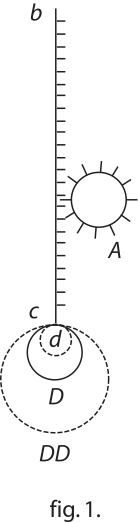
\includegraphics[width=0.1\textwidth]{images/37_3_90r1} 
            \pstart 
           % \begin{wrapfigure}{l}{0.1\textwidth}                    
               % 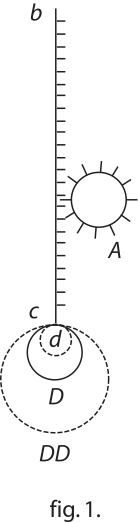
\includegraphics[width=0.1\textwidth]{images/37_3_90r1}
                        %\caption{Bildbeschreibung}
                   %     \end{wrapfigure}
%
    %         \begin{wrapfigure}{l}{0.2\textwidth}                    
        %        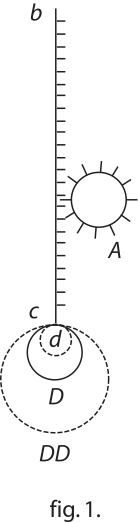
\includegraphics[width=0.2\textwidth]{images/37_3_90r1}
                        %\caption{Bildbeschreibung}
            %            \end{wrapfigure}
                        %@ @ @ Dies ist eine Abstandszeile - fuer den Fall, dass mehrere figures hintereinander kommen, ohne dass dazwischen laengerer Text steht. Dies kann zu einer Fahlermeldung fuehren. @ @ @ \\
            \textso{Sustentatio} est impedimentum intensionis aut restitutionis seu detensionis. \textso{Potentia Contendens} est Elaterium sustentans, et ab Elaterio sustentata. Elaterio scilicet impediente ulteriorem a potentia intensionem, et potentia impediente ulteriorem Elaterii restitutionem. Ut in fig. 2. 
             materia in Tubo comprehensa Elastica esto. Cui incumbat pondus \textit{ab} vel \textit{aabb}. Si pondus in \textit{ab} positum a materiae Elaterio sustinetur, ne ultra descendat, et contra in \textit{aabb} positum a materiae Elaterio levatur, sed non ultra quam in \textit{ab} ubi scilicet potentia Elaterium, et Elaterium potentiam sustinet, \textso{Volumina sustentantia} sunt post absolutam intensionem producta. \textso{Relaxare} est dare libertatem restitutionis.}{\lemma{}\Afootnote{ \textit{ (1) }\ \textso{Vis Elastica}\protect\index{Sachverzeichnis}{vis!elastica|textit} est conatus\protect\index{Sachverzeichnis}{conatus|textit} corporis ad mutandum Volumen. \textso{Volumen} est spatium a corpore occupati. \textso{Volumen Violentum} (\textso{Naturale}) est ad quod mutandum  corpus conatum\protect\index{Sachverzeichnis}{conatus|textit} (non) habet. \textso{Compressio}\protect\index{Sachverzeichnis}{compressio|textit} est status   \textbar\ (vel procuratio status) \textit{ erg.}\ \textbar\  corporis conatum\protect\index{Sachverzeichnis}{conatus|textit} habentis  ad augendum (minuendum) Volumen. \textso{Tensio}\protect\index{Sachverzeichnis}{tensio|textit} est status corporis conatum\protect\index{Sachverzeichnis}{conatus|textit} habentis ad minuendum  Volumen. \textso{Restitutio} est motus corporis ad mutandum Volumen. \textit{ (2) }\  \textso{Vis} [...] impedimentum  \textit{(a)}\ ulterioris \textit{(b)}\ intensionis aut restitutionis seu detensionis.  \textit{(aa)}\ \textso{Potentia intendens}\protect\index{Sachverzeichnis}{potentia!intendens|textit} \textit{(bb)}\ \textso{Potentia Contendens}\protect\index{Sachverzeichnis}{potentia!contendens|textit} \textit{(cc)}\ \textso{Potentia Urgens}\protect\index{Sachverzeichnis}{potentia!urgens|textit} \textit{(dd)}\ \textso{Potentia} [...] ulteriorem  \textbar\ a \textit{ erg.}\ \textbar\ potentia [...] Elaterio \textit{(aaa)}\ sustentatum, leva \textit{(bbb)}\ levatur, [...] restitutionis. \textit{ L}}}\pend% \begin{wrapfigure}{l}{0.2\textwidth}      
           %  \rule[0mm]{0mm}{1mm}
   %     \begin{center}
%             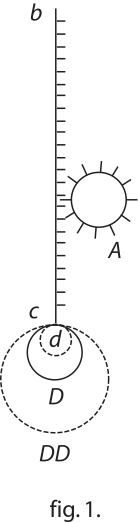
\includegraphics[width=0.2\textwidth]{images/37_3_90r1}               
%                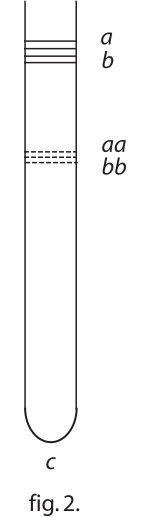
\includegraphics[width=0.22\textwidth]{images/37_3_90r2}
%                 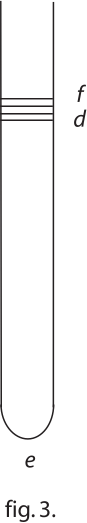
\includegraphics[width=0.13\textwidth]{images/37_3_90r3}
   %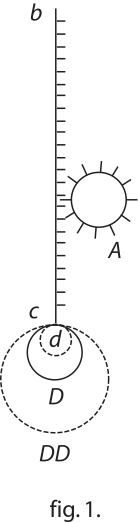
\includegraphics[width=0.19\textwidth]{images/37_3_90r1}               
       %         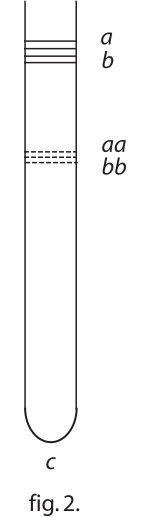
\includegraphics[width=0.21\textwidth]{images/37_3_90r2}
           %      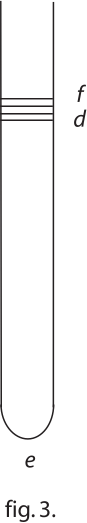
\includegraphics[width=0.12\textwidth]{images/37_3_90r3}
%
                                         %\caption{Bildbeschreibung}
    %                    \end{center}
                  \pstart       \textso{Vis Elastica}\protect\index{Sachverzeichnis}{vis!elastica}\textso{ specifica} est quae speciebus corporum, \edtext{inter}{\lemma{corporum,}\Afootnote{ \textit{ (1) }\ non qu \textit{ (2) }\ inter \textit{ L}}} se collatis aestimatur.\pend 
                  \pstart  (1) Vis Elastica\protect\index{Sachverzeichnis}{vis!elastica} tanta est, quanta est \edtext{potentia contendens est sustendens et sustentata, seu \textso{simul} impediens et impedita}{\lemma{est}\Afootnote{ \textit{ (1) }\ Vis minima  \textit{(a)}\ impediens restitutionem, seu \textit{(b)}\ sustinens Elaterium\protect\index{Sachverzeichnis}{elaterium|textit}  seu impediens restitutionem, vel potentia maxima ab Elaterio\protect\index{Sachverzeichnis}{elaterium|textit} sustentabilis \textit{ (2) }\ potentia [...] impedita \textit{ L}}}.  Nam generatim: omnis potentia tanta est, quantum  est minimum ejus impedimentum sufficiens, \edtext{seu quod impedit et impeditur, aequale est}{\lemma{}\Afootnote{seu quod impedit et impeditur,  \textit{ (1) }\ id est \textit{ (2) }\ aequale est \textit{ erg.} \textit{ L}}}, ut in  Metaphysicis demonstratum\edtext{}{\lemma{}\Afootnote{demonstratum  \textbar\ jam contendens \textit{ erg. u.}\  \textit{ gestr.}\ \textbar\ suppono. \textit{ L}}} suppono.\pend \pstart   %    \begin{wrapfigure}{l}{0.1\textwidth}                    
               % 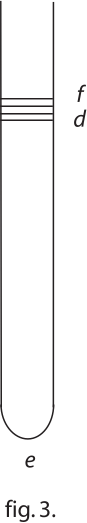
\includegraphics[width=0.1\textwidth]{images/37_3_90r3}\\
                        %\caption{Bildbeschreibung}
                    %    \end{wrapfigure}
                  Pone Rotae \textit{A}  Elaterium\protect\index{Sachverzeichnis}{elaterium} \edtext{(qualis Lamina Ferrea est)}{\lemma{}\Afootnote{(qualis Lamina Ferrea est) \textit{ erg.} \textit{ L}}} esse ita applicatum,  ut restitutione\edtext{}{\lemma{}\Afootnote{restitutione  \textbar\ ejus \textit{ gestr.}\ \textbar\ Elaterii \textit{ L}}} Elaterii\protect\index{Sachverzeichnis}{elaterium} Rotam circumagi necesse sit.  Rotae autem dentis, dentibus columnae \textit{ac} a pondere\protect\index{Sachverzeichnis}{pondus} appenso  detractae\edtext{}{\lemma{}\Afootnote{detractae  \textbar\ vel depressae \textit{ gestr.}\ \textbar\ esse \textit{ L}}} esse insertos, ac proinde  non posse Elaterium\protect\index{Sachverzeichnis}{elaterium} vel minimum restitui,  nisi pondus\protect\index{Sachverzeichnis}{pondus} elevetur tantundem. Esto pondus\protect\index{Sachverzeichnis}{pondus} \textit{d} justo minus, quod scilicet Elaterii\protect\index{Sachverzeichnis}{elaterium} restitutionem non  impediat: Pondus\protect\index{Sachverzeichnis}{pondus} \textit{DD} justo majus, quod scilicet Elaterium\protect\index{Sachverzeichnis}{elaterium}  plus quam impediat, \textso{pondus}\protect\index{Sachverzeichnis}{pondus}\textso{ justum,} \textit{D} quod  sit Elaterii\protect\index{Sachverzeichnis}{elaterium} impedimentum\rule[-2cm]{0cm}{0.5cm} minimum sufficiens, seu  quod auctum sit plus quam sufficiens, \edtext{suffecturum scilicet}{\lemma{sufficiens,}\Afootnote{ \textit{ (1) }\ seu quod sufficiet \textit{ (2) }\ suffecturum scilicet \textit{ L}}}  impediendo etiam fortiori: et imminutum  sufficiens esse \edtext{\edlabel{cess90r1}cesset.}{\lemma{cesset.}\xxref{cess90r1}{cess90r2}\Afootnote{\textit{ (1) }\ Est ergo pondus\protect\index{Sachverzeichnis}{pondus|textit} \textit{D} Elaterio\protect\index{Sachverzeichnis}{elaterium|textit} \textit{ (2) }\  Sunt [...] Elaterii \textit{ L}}} \pend 
                  \pstart Sunt ergo duae potentiae ponderis \textit{D} et Elaterii \textit{A} \edtext{\edlabel{cess90r2}aequales.}{\lemma{aequales.}\xxref{cess90r2}{aequ90r2}\Afootnote{ \textit{ (1) }\ (2) Vis Elastica\protect\index{Sachverzeichnis}{vis!elastica|textit}  \textit{(a)}\ compressorum \textit{(b)}\ corpori intestina fit ex ductu materiae  in motum \textit{ (2) }\  \textso{Vim} corpori intestinam voco,  \textit{(a)}\ quam \textit{(b)}\ cujus principium in  ipso corpore est, seu quae exerceretur aliis corporibus  nihil agentibus \textit{ (3) }\   (2) Vis Elastica\protect\index{Sachverzeichnis}{vis!elastica|textit} totius fit ex additione Virium Elasticarum\protect\index{Sachverzeichnis}{vis!elastica|textit}  omnium partium.  Nam generatim potentia totius  \textit{(a)}\ fit ex \textit{(b)}\ aequalis est  summae ex potentiis partium collectae \textit{ (4) }\  (2)  \textit{(a)}\ Si duae Vires Elasticae\protect\index{Sachverzeichnis}{vis!elastica|textit} comparandae  sunt inter se, ratio ita inibitur \textit{(b)}\ Si duae Vires Elasticae\protect\index{Sachverzeichnis}{vis!elastica|textit}  sustineant Potentias aequales, erunt   \textbar\ inter se \textit{ erg.}\ \textbar\  ut Volumina \textit{ (5) }\  (2) Vires Elasticae Specificae  \textit{(a)}\ erunt inter se  ut Volumina cum aequales potentias contendentes\protect\index{Sachverzeichnis}{potentia!contendens|textit} sustinent \textit{(b)}\ sunt inter se ut Volumina  \textit{(aa)}\   \textbar\ Residua \textit{ erg.}\ \textbar\ , caeteris paribus \textit{(bb)}\ Residua, caeteris paribus \textit{(cc)}\ sustentantia, caeteris paribus \textit{ L}}}
                  \pend  
% Zeitz auskommentiert                  \begin{center}
%           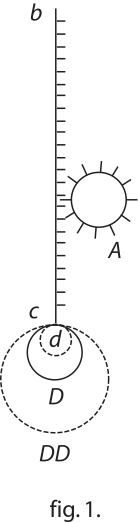
\includegraphics[width=0.155\textwidth]{images/37_3_90r1}               
%                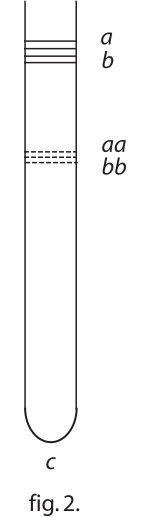
\includegraphics[width=0.175\textwidth]{images/37_3_90r2}
%                 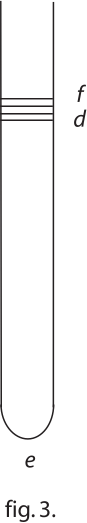
\includegraphics[width=0.1\textwidth]{images/37_3_90r3}
%   %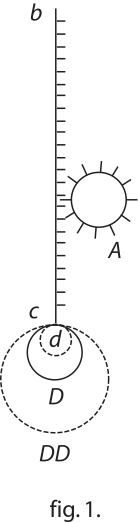
\includegraphics[width=0.19\textwidth]{images/37_3_90r1}               
%       %         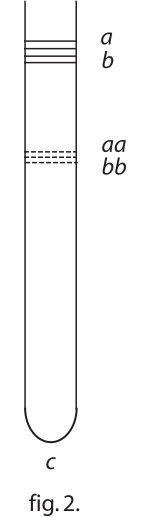
\includegraphics[width=0.21\textwidth]{images/37_3_90r2}
%           %      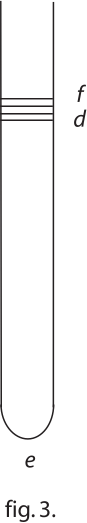
\includegraphics[width=0.12\textwidth]{images/37_3_90r3}
%%
%                                         %\caption{Bildbeschreibung}
%                       \end{center}
            \pstart (2) Vires Elasticae Specificae sunt inter se ut Volumina sustentantia, caeteris paribus seu duae Vires Elasticae\protect\index{Sachverzeichnis}{vis!elastica} Specificae ita comparabuntur:  Si \edtext{\edlabel{aequ90r2}in fig. 2. 3.}{\lemma{}\Afootnote{in fig. 2. 3. \textit{ erg.} \textit{ L}}}  duo corpora Elastica\protect\index{Sachverzeichnis}{corpus!elasticum} \edtext{\textit{bc} et \textit{de}}{\lemma{}\Afootnote{\textit{bc} et \textit{de} \textit{ erg.} \textit{ L}}} diversarum specierum \edtext{ut aeris aut lanae, vel aeris ordinarii aut rari pressive}{\lemma{}\Afootnote{ut   \textbar\ aeris aut lanae, vel \textit{ erg.}\ \textbar\  aeris ordinarii aut rari pressive \textit{ erg.} \textit{ L}}} eodem \edtext{seu aequali}{\lemma{}\Afootnote{seu aequali \textit{ erg.} \textit{ L}}} pondere\protect\index{Sachverzeichnis}{pondus} seu eadem \edtext{potentia intendente}{\lemma{potentia}\Afootnote{ \textit{ (1) }\ contendente \textit{ (2) }\ intendente \textit{ L}}} \edtext{\textit{ab} vel \textit{fd}}{\lemma{}\Afootnote{\textit{ab} vel \textit{fd} \textit{ erg.} \textit{ L}}}  urgeantur, erunt \edtext{enim}{\lemma{}\Afootnote{enim \textit{ erg.} \textit{ L}}} inter se, ut volumina \edtext{\textit{bc} et \textit{de}}{\lemma{volumina}\Afootnote{ \textit{ (1) }\ sustinentia  seu \textit{ (2) }\ \textit{bc} et \textit{de} \textit{ L}}}  post absolutam compressionem\protect\index{Sachverzeichnis}{compressio} residua, (aut post  absolutam tensionem\protect\index{Sachverzeichnis}{tensio} \edtext{producta).\edlabel{prod90v1}}
                  {\lemma{producta).}\xxref{prod90v1}{prod90v2}\Afootnote{ \textit{ (1) }\ Quia si  eadem potentia in diversa obstacula diversos habet effectus, erunt obstacula ut effectus, ut in Metaphysica demonstratum suppono. Sed quia tales Metaphysicas,  quibus ejusmodi propositiones demonstrentur, malo publico non habemus, hoc loco obiter demonstrabo. \textit{ (2) }\ Esto potentia \textit{A} obstaculum \textit{B}  \textit{(a)}\ effectus\protect\index{Sachverzeichnis}{effectus|textit} constat  ajo \textit{(b)}\ constat effectum\protect\index{Sachverzeichnis}{effectus|textit} esse \textit{A-B}. Esto aliud obstaculum \textit{C}  effectus in hoc, erit \textit{A-C}. Jam 
\protect\begin{tabular}{ccccc}
\textit{A - B}&est ad&\textit{A - C}&ut&\textit{B ad C.}\\
10 - 4&&10 - 5&&4 ad 5\\
6&&5&&
\protect\end{tabular}
Nam in numeris  Error ergo seu falsa propositio  utcunque speciosa. \textit{ (3) }\  Nam Vires Elasticae\protect\index{Sachverzeichnis}{vis!elastica|textit} simpliciter  \textit{(a)}\ materiae \textit{bc} et \textit{(b)}\ tum materiae \textit{bc} tum \textit{de} sunt  aequales per prop. 1. Sustinent enim aequales potentias. \textit{ (4) }\   Hoc sic ostendo, augeatur   \textbar\ (vel minuatur) \textit{ erg.}\ \textbar\ utrobique [...] pressionem  \textbar\ seu post aequilibrium\protect\index{Sachverzeichnis}{aequilibrium|textit} \textit{ erg.}\ \textbar\ producta, [...] aequalia. \textit{ L}}} 